\chapter{Classification: Basic Concepts, Decision Trees, and Model Evaluation}

	

	\clearpage

	\section{Preliminary}

		The input data for a classification task is a collection of records.
		Each record, also known as an instance or example, is characterized
		by a tuple ({\bf x}, y), where {\bf x} is the {\bf attribute set} and
		{\bf y} is a special attribute called a {\bf classification class (class label)}.

		The attribute set can be descrete and continuous, but the class label
		is always a descrete value. 

		{\bf Definition 1:} classification is the task of
		learning a {\bf taget function f} that maps each attribute set {\bf x}
		to one of the predifined class labels y.

		{\bf Definition 2:} classificarion is the task of assigning objects to one of several
		predefined categories, or in other words, classification is the task
		of mapping an input attribute set x into its class label y.

	\begin{figure}[H]
		\centering
		\includegraphics[width=\textwidth]{pics/classification2.png}
	\end{figure}

		The target function is also known as a {\bf classification model}.
		A classification model is useful for the following purposes:
			\begin{itemize}
				\item {\bf Descriptive Modeling:} can use the class label that
				explains what features defines a object (class label $\rightarrow$ features)				
				\item {\bf Predictive Modeling:} a classification model can be
				used to predict the class label of unknown records. (features $\rightarrow$ class label)
			\end{itemize}

	\clearpage	
	\section{General Approach to Solving a Classification Problem}

		{\bf Learning algorithm:} identifies a model that best fits the relationships
		between the attribute set and class label of input data. Examples of learning 
		algorithms are: decision tree classifiers, rule-based classifiers, neural networks, 
		support vector machines, and naive Bayes classifiers. 

		{\bf Traing set:} consists of records whose class labels are known must be provided.
		The training set is used to build a classification model, which is subsequently applied
		to the test set.

		{\bf Test set:} consists of records with unknown class labels.

		\begin{figure}[H]
			\includegraphics[width=\textwidth]{pics/classification3.png}
			\caption{General approach to solving classification problem}
		\end{figure}

		{\bf Confusion matrix:} evaluation of classification model is based on the coounts of
		test records correctly and incorrectly predicted by the model. The results are known
		as a confusion matrix. The perfromance can be calculated with accuracy or error rate
		which uses the numbers from the confusion matrix. 

		\begin{table}[H]
		\centering
			\begin{tabular}{| l | l | l | l |}
				\hline
				\multicolumn{2}{| l |}{\multirow{2}{*}{ }} & \multicolumn{2}{| l |}{Predicted class} \\ \cline{3-4} 
				 & & Class = 1 & Class = 0 \\ \hline
				\multirow{2}{*}{Actual class} & Class = 1 & $f_{11}$ & $f_{10}$ \\ \cline{2-4}
					& Class = 0 & $f_{01}$ & $f_{00}$ \\ \hline

			\end{tabular}
			\caption{Confusion matrix for a 2-class problem.}
		\end{table}

		\begin{equation}
			Accuracy = \frac{Number of correct predictions}{Total number of predictions} =
			\frac{f_{11} + f_{00}}{f_{11} + f_{10} + f_{01} + f_{00}}
		\end{equation}
		\begin{equation}
			Error rate = \frac{Number of wrong predictions}{Total number of predictions} =
			\frac{f_{10} + f_{01}}{f_{11} + f_{10} + f_{01} + f_{00}}
		\end{equation}
	\clearpage
	\section{Decision Tree}

		We can solve a classification problem by asking a series of carefully
		crafted {\bf questions} about the attributes of the test record. 
		Each time we recieve an answer, a follow-up question is asked until
		we reach a conclusion about the class label of the record. The series
		of question and their possible answers can be organaized in the form of
		a decision tree, which is a hierarchical structure consisting of nodes
		and directed edges.

		\begin{itemize}
			\item {\bf A root node} has no incoming edges and zero or more outgoing edges
			\item {\bf Internal nodes}, each of which has exactly one incoming edge and 
			two or more outgoing edges. An internal node is a new question.  
			\item{\bf Leaf/terminal nodes} , each of which has exactly one incoming edge
			and no icoming edges. Is a class label. If a leaf node is reached, you got the
			conclusion. 
		\end{itemize}

		\begin{figure}[H]
			\centering
			\includegraphics[scale=0.4]{pics/decision.png}
		\end{figure}

		There is many ways to construct a decision tree. There is many known algorithms to
		do this: Hunt's algorithm, ID3, C4.5 and CART. 
		Hunt's algorithm is a more general description, and ID3 is a more specific/detailed
		version of the Hunt's algorithm (basicly the same).

\clearpage
		\subsection*{Hunt's algorithm} 
		Let $D_{t}$ be the set of training records that are 
		associated with node t and y = {$y_{1}, y_{2}, ...., y_{c}$} be the class labels. 
		This is a recursive definition of Hunt's algorithm:
		\begin{enumerate}
			\item If all the records in $D_{t}$ belongs to the same class $y_{t}$, then
			t is a leaf node labeled as $y_{t}$
			\item If $D_{t}$ contains records that belong to more than one class, an
			attribute test condition is selected to partiotion the records into smaller
			subsets. A child node is created for each outcome of the test condition and 
			the records in $D_{t}$ are distributed to the childdren based on the outcomes. 
			The algorithm is then recursively applied to each child node. 
		\end{enumerate} 

		Hunt's algorithm will work if every combination of attribute values is present
		in the training data and each combination has a unique class label. 
		These assuptions are too stringent for use in most practical situations.

		{\bf Additional conditions are needed to handle the following cases:}

		\begin{enumerate}
			\item {\bf Empty child nodes:} in this case the node is declared a leaf
			node with the same class label as the majority class of training records
			associated with its parent node. 
			\item{\bf Identical attribute values:} if all the records associated with
			$D_{t}$ have identical attribute values (expect for the class label), then
			it is not possible to split these records any further. In this case, the node is
			declared a leaf node with the same class label as the majority class of 
			training records associated with this node.
		\end{enumerate}

		{\bf Design issues of decision trees}
			\begin{itemize}
				\item How should the training records be split?
				\item How should the splitting procedure stop?
			\end{itemize}

	\subsection{Methods for Expressing Attribute Test Conditions}

		{\bf Binary Attributes:} Have only 2 potential outcomes.

		{\bf Nominal Attributes:} Can have many values, so you can either have
		a multiway split (split for each value) or have a binary split by grouping
		the values. 

		{\bf Ordinal Attributes:} ordinal values can be handeled in the same way as
		nominal attributes, except that the values have an order. It does not make
		sense to combine the values "small, large" and "medium, extra large". To do
		a binary split, you would have to group feks "small, medium" and "large, extra large".

		{\bf Continuous Attributes:} here you can use a test condition expressed as a
		comparison with binary outcomes (A $<$ v or A$>$v), or a range query with outcomes 
		with multiple values. 

	\clearpage
	\subsection{Measures for Selecting the Best Split}
		$p(i|t)$ is the fraction of records belonging  to class i at a given node t.		
		c is the number of classes.
		Here are three different impurity measures: 
		\begin{equation}
			Entropy(t) = -\sum_{i=0}^{c-1} p(i|t)log_{2}p(i|t)
		\end{equation}

		\begin{equation}
			Gini(t) = 1 - \sum_{i=0}^{c-1}[p(i|t)]^{2}
		\end{equation}
		\begin{equation}
			Classification error(t) = 1 - max_{i}[p(i|t)]
		\end{equation}

		\begin{table}[H]
		\centering
		\begin{tabular}{ l l }
			 \hline
			\begin{tabular}{|l|l|}
				\hline
				\rowcolor{gray}
				Node $N_{1}$ & Count \\ \hline
				Class=0 & 0 \\ \hline
				Class=1 & 6 \\ \hline
			\end{tabular}
		& 
			\begin{tabular}{l}
				Gini = 1 - $(0/6)^{2}$ - $(6/6)^{2}$ = 0 \\
				Entropy = -(0/6)$log_{2}$(0/6) - (6/6)$log_{2}$(6/6) = 0 \\ 
				Error = 1-$max[(0/6), (6/6)] = 0$ \\
			\end{tabular}

 		\\ \hline

			\begin{tabular}{|l|l|}
				\hline
				\rowcolor{gray}
				Node $N_{2}$ & Count \\ \hline
				Class=0 & 1 \\ \hline
				Class=1 & 5 \\ \hline
			\end{tabular}
		&
			\begin{tabular}{l}
				Gini = 1 - $(1/6)^{2}$ - $(5/6)^{2}$ = 0.278  \\
				Entropy = -(1/6)$log_{2}$(1/6) - (5/6)$log_{2}$(5/6) = 0.650  \\
				Error = 1-$max[(1/6), (6/6)] = 0.167$
			\end{tabular}	
		\\ \hline

			\begin{tabular}{|l|l|}
				\hline
				\rowcolor{gray}
				Node $N_{3}$ & Count \\ \hline
				Class=0 & 3 \\ \hline
				Class=1 & 3 \\ \hline
			\end{tabular}
		& 
			\begin{tabular}{l}
				Gini = 1 - $(3/6)^{2}$ - $(3/6)^{2}$ = 0.5 \\
				Entropy = -(3/6)$log_{2}$(3/6) - (3/6)$log_{2}$(3/6) = 1 \\
				Error = 1-$max[(3/6), (3/6)] = 0.5$ 
			\end{tabular}
		\\ \hline
		\end{tabular}
		\end{table}

		To determine how well a test condition performs, we need to compare the 
		degree of impurity of the parent node (before splitting) with the degree
		of impurity of the child nodes (after splitting). The larger the difference,
		the better the test condition. The gain $\Delta$, is a criterion that can 
		be used to determine the goodness of a split. 

			\begin{equation}
				\Delta = I(parent) - \sum_{j=1}^{k} \frac{N(v_{j})}{N}I(v_{j})
			\end{equation}

		I(.) is the impurity measure of a given node, N is the total number
		of records at the parent node, k is the number of attribute values, 
		and N($v_{j}$) is the number of records associated with the child node, $v_{j}$.
		When entropy is used as the impurity measure in equation 4.6, the difference
		in entropy is known as the {\bf information gain}, $\Delta_{info}$.

		\subsection*{Example of calculation with Gini}
		\begin{figure}[H]
			\centering
			\includegraphics[scale=0.25]{pics/gini.png}
			\caption{Example of splitting binary attributes by using gini}
		\end{figure}

		{\bf Gain ratio:} in C4.5 decision tree algorithm, a splitting criterion known
		as gain ratio is used to determine the goodness of a split. The criterion is
		defined as follows:

		\begin{equation}
			Gain\;ratio = \frac{\Delta_{info}}{Split\;Info}
		\end{equation}

		\begin{equation}
			\Delta_{info} = Information\;gain = Entropy(Parent) - Entropy(Node)
		\end{equation}

		\begin{equation}
			Split\;Info = - \sum_{i=1}^{k} P(v_{i})log_{2}P(v_{i})
		\end{equation}

		k is the total number of splits.

		\clearpage
		\section{Overfitting and undefitting}

		The errors committed by a classification model are generally divided into
		two types: {\bf training errors} and {\bf generalization errors}.
		Training error, also known as {\bf resubstitution error} or {\bf apparent error}, 
		is the number of misclassification errors committed on training records, wheras
		generalization error is expected error of the model on previously unseen records. 

		A good classification model must not only fit the training data well, it must
		also accurately classify records it has never seen before. In other words, 
		a good model must have low training error as well as low generalization error. 
		This is important because a model that fits the training data too well can 
		have a poorer generalization error than a model with a higher training error.
		Such a situation is known as model {\bf overfitting}.

		You often get high training and error rates of the model when the size of the
		tree is very small or the training set is too small. This situation is known 
		as {\bf underfitting}.

		\begin{figure}[H]
			\centering
			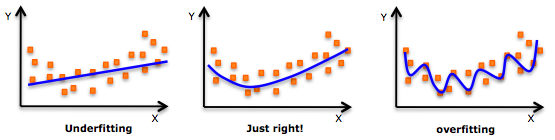
\includegraphics[width=\textwidth]{pics/fitting.png}
		\end{figure}

		{\bf Causes of overfitting:}
		\begin{itemize}
			\item Overfitting due to presence of noise
			\item Overfitting due to lack of representative samples
		\end{itemize}

		\subsection{Handling overfitting in decision tree induction}

		This section presents two strategies for avoiding model overfitting 
		in the context of decision tree induction. 

		{\bf Prepruning (early stopping rule):} in this approach, the tree growing
		algorithm is halted before generating a fully grown tree that perfectly
		fits the entire training data. To do this, a more restrictive stopping condition
		must be used e.g., stop expanding a leaf node when the observed gain in
		impurity measure (or improvement in the estimated generalization error) falls
		below a certain threshold. 

		{\bf Post-pruning:} in this approach, the decision tree is initially grown 
		to its maximum size. This is followed by a tree-pruning step, which proceeds
		to trim the fully grown tree in a bottom-up fashion. Trimming can be done by
		replacing a subtree with (1) a new leaf node whose class label is determined
		from the majority class of records affiliated with the subtree, or (2) the most
		frequently used branch of the subtree. 

		\begin{figure}[H]
			\centering
			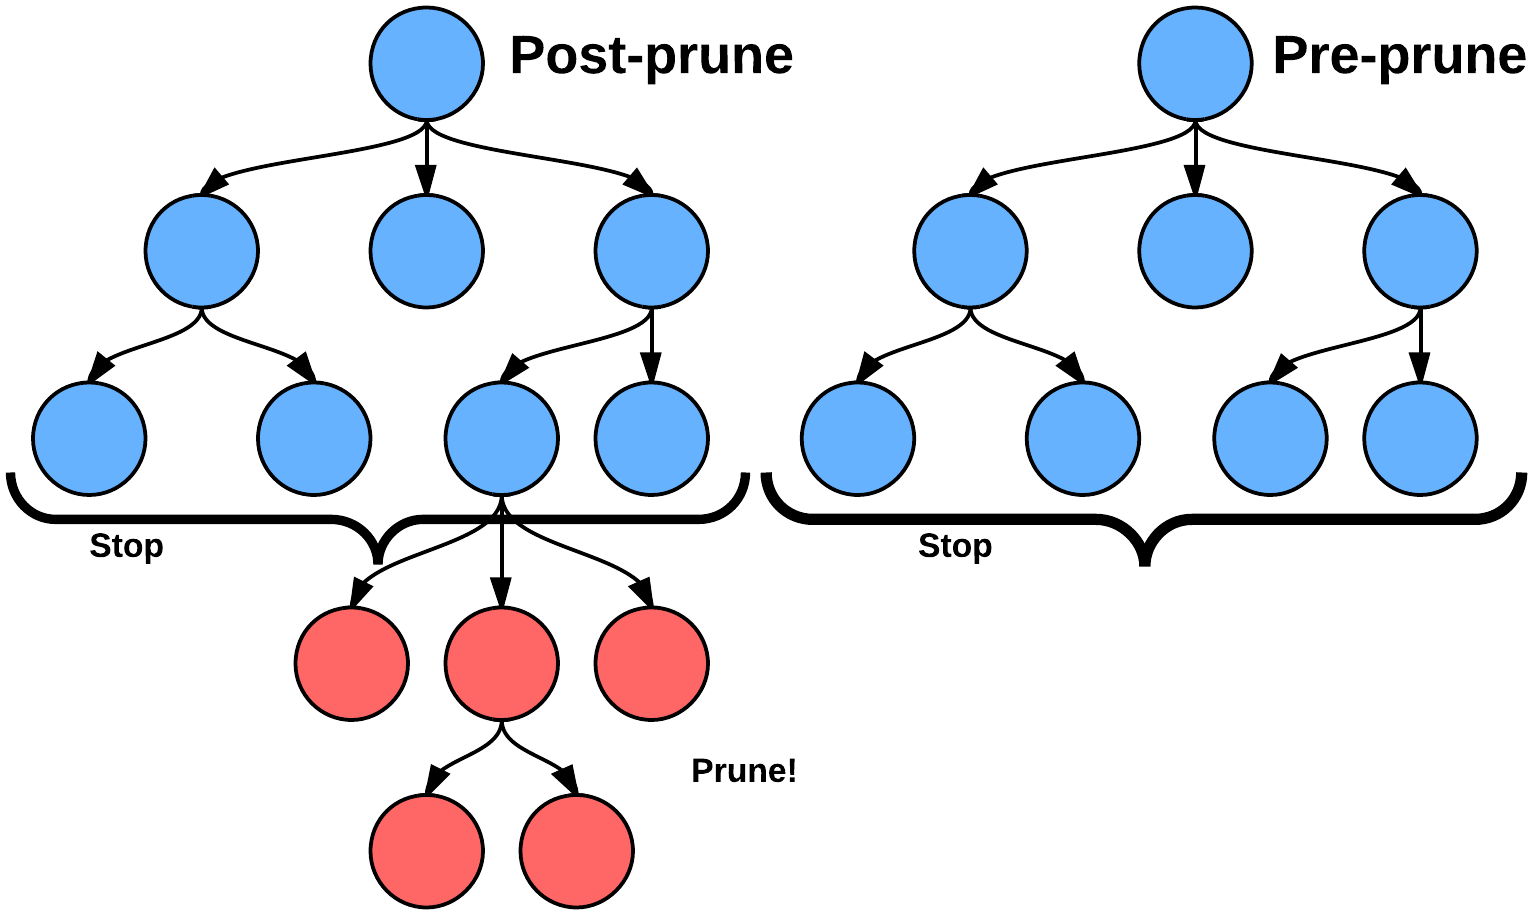
\includegraphics[width=\textwidth]{pics/prepostprune.png}
			\caption{Pre-pruning and post-pruning of decision tree}
		\end{figure}


	\clearpage
	\section{Evaluating the Performance of a Classifier}

		This section reviews some of the methods commonly used to evaluate the 
		performance og a classifier. 

		\subsection*{Holdout Method}
		In the holdout method, the original data with labeled examples is
		partitioned into two disjoint sets, called the training and the test set.
		A classification model is then introduced from the training set and its
		performance is evaluated on the test set. 

		\subsection*{Random Subsampling}
		The holdout method can be repeated several times to improve the estimation
		of a classifier's performance. This approach is known as random subsampling.
		One problem is that it does not have control over the number of times
		each record is used for testing and training. 

		\subsection*{Cross-Validation}
		An alternative to random subsampling is cross-validation. In this approach, 
		each record is used the same number of times for training and exactly once 
		for testing. To illustrate this method, suppose we partition the data into
		two equal-sized subsets. First, we choose one of the subsets for training 
		and the other for testing. We then swap the roles of the subsets so that
		the previous training set becomes the test set and vice versa. This approach
		is called a {\bf two-fold cross-validation}. The total error is obtained by summing
		up the errors for both runs. In this example, each record is exactly once 
		for training and once for testing. The {\bf k-fold cross-validation} method
		generalizes this approach by segmenting the data into k equal-sized partitions.
		During each run, one of the partitions is chosen for testing, while the rest
		of them are used for training. This procedure is repeated k times so that
		each partition is used for testing exactly once. Again, the total error is
		found by summing up the errors for all k runs. 
		A special case of the k-fold cross-validation method sets k=N, the size of 
		the data set. In this so called {\bf leave-one-out} approach, each test set 
		contains only one record. 

		\subsection*{Bootstrap}
		The methods represented so far assume that the training records are sampled
		{\bf without replacement}. As a result, there are no duplicate records in the training
		and test sets. In the bootstrap approach, the training records are sampled 
		{\bf with replacement};i.e., a record already chosen for training is put back into
		the original pool or records so that it is equally likely to be redrawn. 
		It will often be the case that a bootstrap  sample size of N contains 
		about 63.2\% of the records in the original data. 
		Records that are not included in the bootstrap sample become part of the
		test set (ca 46.7\% of the original data).
		The model induced from the training set is then applied to the test set
		to obtain an estimate of the accuracy of the bootstrap sample, $e_{i}$.
		Then the sampling procedure is then repeated b times to generate b bootstrap
		samples. 

		\clearpage

		\begin{figure}[H]
			\centering
			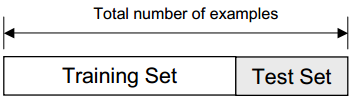
\includegraphics[scale=0.5]{pics/holdout.png}
			\caption{Holdout Method}
		\end{figure}

		\begin{figure}[H]
			\centering
			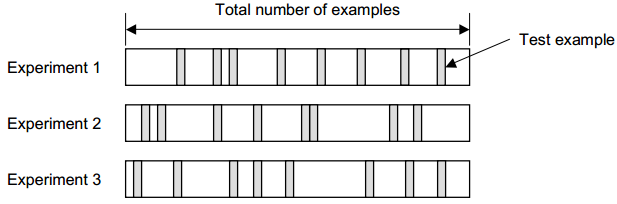
\includegraphics[scale=0.5]{pics/randomsubsampling.png}
			\caption{Random Subsampling}
		\end{figure}

		\begin{figure}[H]
			\centering
			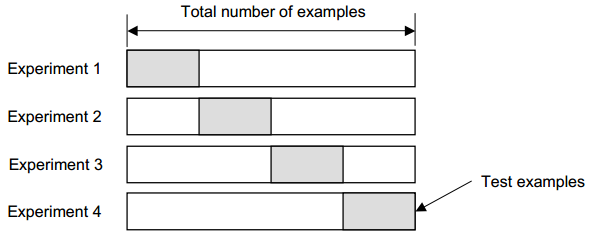
\includegraphics[scale=0.5]{pics/kfold.png}
			\caption{Cross-Validation}
		\end{figure}

		\begin{figure}[H]
			\centering
			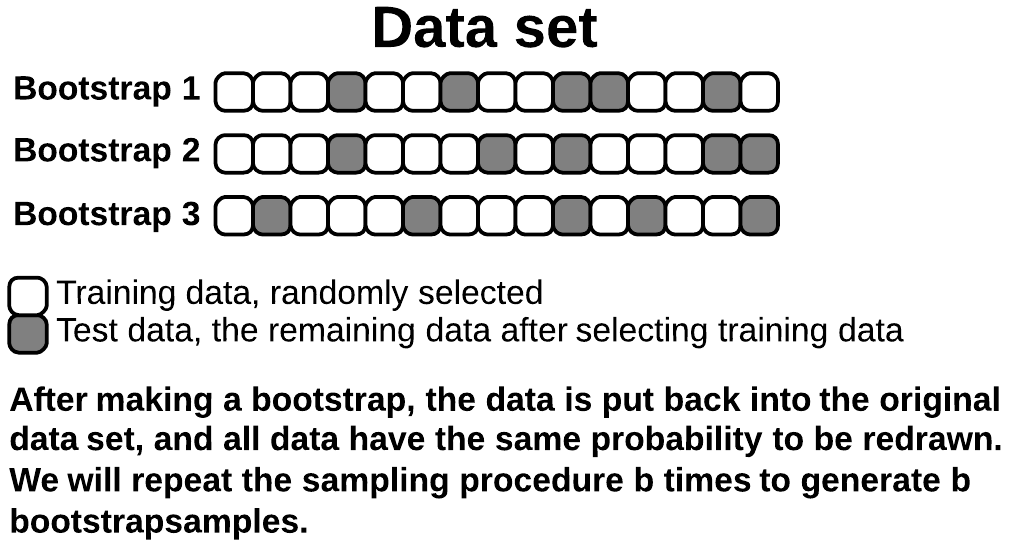
\includegraphics[scale=0.3]{pics/bootstrap.png}
			\caption{Bootstrap}
		\end{figure}

